
\section{Análisis de resultados}

En esta sección se muestran y estudian los resultados tras la resolución de la flexión simple propuesta. En particular, tras la deformación, se determinan la tensión y deformación en el plano de la galga, el desplazamiento en el punto de aplicación de la carga, la carga máxima aplicable y los coeficientes de seguridad. Finalmente se hace un estudio de malla, donde se comparan los resultados de la simulación inicial con los resultados obtenidos para una malla más burda y para una malla más fina. En las Secciones \ref{sec:tension_en_la_galga} a \ref{sec:carga_maxima_aplicable_y_coeficiente_de_seguridad} se utiliza una malla con $2.0 \ \milli\meter$ de tamaño máximo de elemento de malla.

\subsection{Tensión en la galga} \label{sec:tension_en_la_galga}

En la situación representada en la Figura \ref{fig:planteamiento}, la tensión analítica viene dada por \cite{manualPractica1}:
\begin{equation} \label{eq:tension_analitica_galga}
    \sigma_{g} = 6 \frac{P L_g}{b t^2}
\end{equation}
Sustituyendo por los valores recogidos en la Tabla \ref{tab:datos}, se obtiene la siguiente tensión:
\[
    \sigma_{g,\text{analítica}} = 
    6 \, \frac{26 \ \newton \cdot 190 \ \milli\meter}{42 \ \milli\meter \cdot (3.5 \ \milli\meter)^2} = 
    57.609 \ \mega\pascal
\]
A fin de determinar las tensiones numéricamente, se corta la probeta con el plano de vector normal $\hat{n} = (1, 0, 0)$ que pasa por la galga en $x = 50 \ \milli\meter$, a saber, el plano de ecuación $\Pi \colon x = 50 \ \milli\meter$. En las Figuras \ref{fig:stress_vector_x_20}, \ref{fig:stress_vector_y_20} y \ref{fig:stress_vector_z_20} se muestran las distribuciones de tensiones en la sección resultante del corte en las direcciones normal $xx$ $(\sigma_{11})$, y en las dos direcciones tangenciales $xy$ $(\sigma_{12})$ y $xz$ $(\sigma_{13})$, respectivamente. Asimismo, en la Figura \ref{fig:stress_vector_magnitude_20} se representa la norma del vector tensión asociado al plano de corte $(\vec{\sigma}_{e_1})$.

\begin{figure}[H]
    \centering
    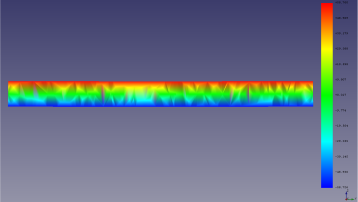
\includegraphics[width=\textwidth]{figures/resultados/stress_vector_x_20.pdf}
    \caption{Distribución de tensión normal $xx$ $(\sigma_{11})$ en el plano de corte $\Pi$. Rango de la escala: $[-58.726, \ 58.760] \ \mega\pascal$. Tamaño máximo de un elemento de malla: $2.0 \ \milli\meter$.}
    \label{fig:stress_vector_x_20}
\end{figure}

\begin{figure}[H]
    \centering
    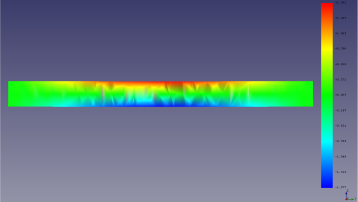
\includegraphics[width=\textwidth]{figures/resultados/stress_vector_y_20.pdf}
    \caption{Distribución de tensión tangencial $xy$ $(\sigma_{12})$ en el plano de corte $\Pi$. Rango de la escala: $[-1.577, \ 1.591] \ \mega\pascal$. Tamaño máximo de un elemento de malla: $2.0 \ \milli\meter$.}
    \label{fig:stress_vector_y_20}
\end{figure}

\begin{figure}[H]
    \centering
    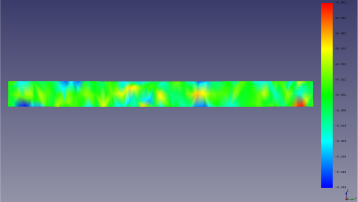
\includegraphics[width=\textwidth]{figures/resultados/stress_vector_z_20.pdf}
    \caption{Distribución de tensión tangencial $xz$ $(\sigma_{13})$ en el plano de corte $\Pi$. Rango de la escala: $[-0.059, \ 0.062] \ \mega\pascal$. Tamaño máximo de un elemento de malla: $2.0 \ \milli\meter$.}
    \label{fig:stress_vector_z_20}
\end{figure}

\begin{figure}[H]
    \centering
    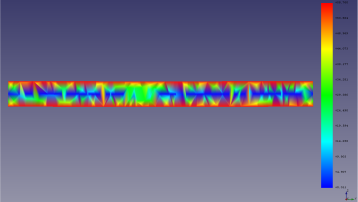
\includegraphics[width=\textwidth]{figures/resultados/stress_vector_magnitude_20.pdf}
    \caption{Distribución de la norma de la tensión $(\norm{\vec{\sigma}_{e_1}})$ en el plano de corte $\Pi$. Rango de la escala: $[0.011, \ 58.760] \ \mega\pascal$. Tamaño máximo de un elemento de malla: $2.0 \ \milli\meter$.}
    \label{fig:stress_vector_magnitude_20}
\end{figure}

Como puede observarse, los máximos de las componentes tangenciales $\sigma_{12}$ y $\sigma_{13}$ en valor absoluto son uno y dos órdenes de magnitud menores, respectivamente, al valor máximo de la componente normal $\sigma_{11}$ en valor absoluto. Por este motivo, $\sigma_{12}$ y $\sigma_{13}$ solamente son relevantes para el cálculo de $\norm{\vec{\sigma}_{e_1}}$ en la zona central de la sección, es decir, cuando $z \approx t / 2$; mientras que cuando $z = 0$ o $z = t$, se puede aproximar por la componente normal, es decir, $\norm{\vec{\sigma}_{e_1}} \approx \abs{\sigma_{11}}$.

Para reducir errores, el valor de la tensión en la posición de la galga se promediará con los valores de la cara superior e inferior:
\begin{equation}
    \sigma_{g,\text{numérica}} = 
    \frac{\abs{\sigma_\text{superior}} + \abs{\sigma_\text{superior}}}{2}
\end{equation}
La tensión en la cara superior es $\sigma_\text{superior} = 57.760 \ \mega\pascal$ y en la inferior $\sigma_\text{inferior} = -58.726 \ \mega\pascal$, de modo que
\[
    \sigma_{g,\text{numérica}} = 
    \frac{58.760 \ \mega\pascal + 58.726 \ \mega\pascal}{2} = 58.743 \ \mega\pascal
\]

El error relativo entre los valores analítico y numérico se obtiene comparando la diferencia entre ambos con el valor analítico:
\begin{equation} \label{eq:error_relativo_tension}
    \text{error}[\%] = 
    100 \ 
    \frac{
    \abs{\abs{\sigma_{g,\text{analítica}}} - \abs{\sigma_{g,\text{numérica}}}}}{\abs{\sigma_{g,\text{analítica}}}}
\end{equation}

Sustituyendo en \eqref{eq:error_relativo_tension}, se obtiene el siguiente error relativo:
\[
    \text{error}[\%] = 
    100 \ 
    \frac{\abs{57.609 \ \mega\pascal - 58.743 \ \mega\pascal}}{57.609 \ \mega\pascal} = 
    1.968 \%
\]

El error relativo máximo aceptable no está establecido uniformemente. Por ejemplo, en el campo de la economía, si se resuelve numéricamente la ecuación de Black--Scholes \cite{salsa2016partial}, que modela los precios de derivados financieros, un error relativo del $1 \%$ comparando con la solución analítica puede considerarse inaceptable. No obstante, para la flexión simple, puede fijarse un error relativo máximo del $5 \%$. En consecuencia, el error obtenido de $1.968 \%$ es aceptable, es decir, la solución analítica y la numérica concuerdan.

\subsection{Deformación en la galga}

Para el cálculo analítico de la deformación nominal se emplea la ley de Hooke para estados tensionales unidireccionales \cite{manualPractica1},
\begin{equation}
    \varepsilon_g = \frac{\sigma_g}{E}
\end{equation}
donde $\sigma_g$ es la tensión dada por \eqref{eq:tension_analitica_galga} y $E$ es el módulo de Young del material. Sustituyendo por la tensión analítica previamente encontrada, se tiene que:
\[
    \varepsilon_{g,\text{analítica}} = 
    \frac{57.609 \ \mega\pascal}{69 \ \giga\pascal} = 
    8.3491 \times 10^{-4} 
\]

En cuanto a las deformaciones numéricas, nuevamente se corta la probeta con el plano de ecuación $\Pi \colon x = 50 \ \milli\meter$. En las Figuras \ref{fig:strain_vector_x_20}, \ref{fig:strain_vector_y_20} y \ref{fig:strain_vector_z_20} se representan las deformaciones en la sección resultante del corte en las direcciones normal $xx$ $(\varepsilon_{11})$ y en las dos direcciones tangenciales $xy$ $(\varepsilon_{12})$ y $xz$ $(\varepsilon_{13})$. En la Figura \ref{fig:strain_vector_magnitude_20} se representa la norma del vector deformación asociado al plano de corte $(\vec{\varepsilon}_{e_1})$.

Se observa cómo, en la cara superior, la componente de deformación $\varepsilon_{11}$ es positiva, mientras que en la cara inferior es negativa. Por el contrario, las componentes $\varepsilon_{12}$ y $\varepsilon_{13}$ son negativas en la cara superior y positivas en la inferior. Esto implica que la sección resultante del corte, la cara superior se ``alarga'' en dirección $x$ y ``contrae'' en direcciones $y$ y $z$; en tanto que la cara inferior se ``contrae'' en dirección $x$ y ``alarga'' en direcciones $y$ y $z$. 

En las caras superior e inferior de la sección se tiene que $\abs{\varepsilon_{11} / \varepsilon_{12}} \approx 3$ y  $\abs{\varepsilon_{11} / \varepsilon_{13}} \approx 3$, por lo que las tres componentes del vector $\vec{\varepsilon}_{e_1}$ están en el mismo orden de magnitud. Así pues, la aproximación $\norm{\vec{\varepsilon}_{e_1}} \approx \abs{\varepsilon_{11}}$ no es buena, a diferencia de con las tensiones.

\begin{figure}[H]
    \centering
    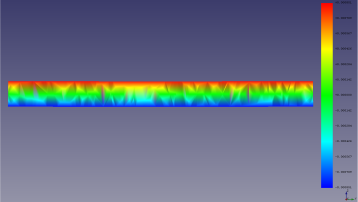
\includegraphics[width=\textwidth]{figures/resultados/strain_vector_x_20.pdf}
    \caption{Distribución de la deformación normal $xx$ $(\varepsilon_{11})$ en el plano de corte $\Pi$. Rango de la escala: $[-8.51, \ 8.51] \times 10^{-3}$. Tamaño máximo de un elemento de malla: $2.0 \ \milli\meter$.}
    \label{fig:strain_vector_x_20}
\end{figure}

\begin{figure}[H]
    \centering
    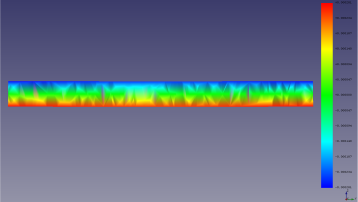
\includegraphics[width=\textwidth]{figures/resultados/strain_vector_y_20.pdf}
    \caption{Distribución de la deformación tangencial $xy$ $(\varepsilon_{12})$ en el plano de corte $\Pi$. Rango de la escala: $[-2.81, \ 2.81] \times 10^{-3}$. Tamaño máximo de un elemento de malla: $2.0 \ \milli\meter$.}
    \label{fig:strain_vector_y_20}
\end{figure}

\begin{figure}[H]
    \centering
    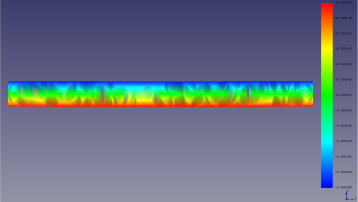
\includegraphics[width=\textwidth]{figures/resultados/strain_vector_z_20.pdf}
    \caption{Distribución de la deformación tangencial $xz$ $(\varepsilon_{13})$ en el plano de corte $\Pi$. Rango de la escala: $[-2.86, \ 2.86] \times 10^{-3}$. Tamaño máximo de un elemento de malla: $2.0 \ \milli\meter$.}
    \label{fig:strain_vector_z_20}
\end{figure}

\begin{figure}[H]
    \centering
    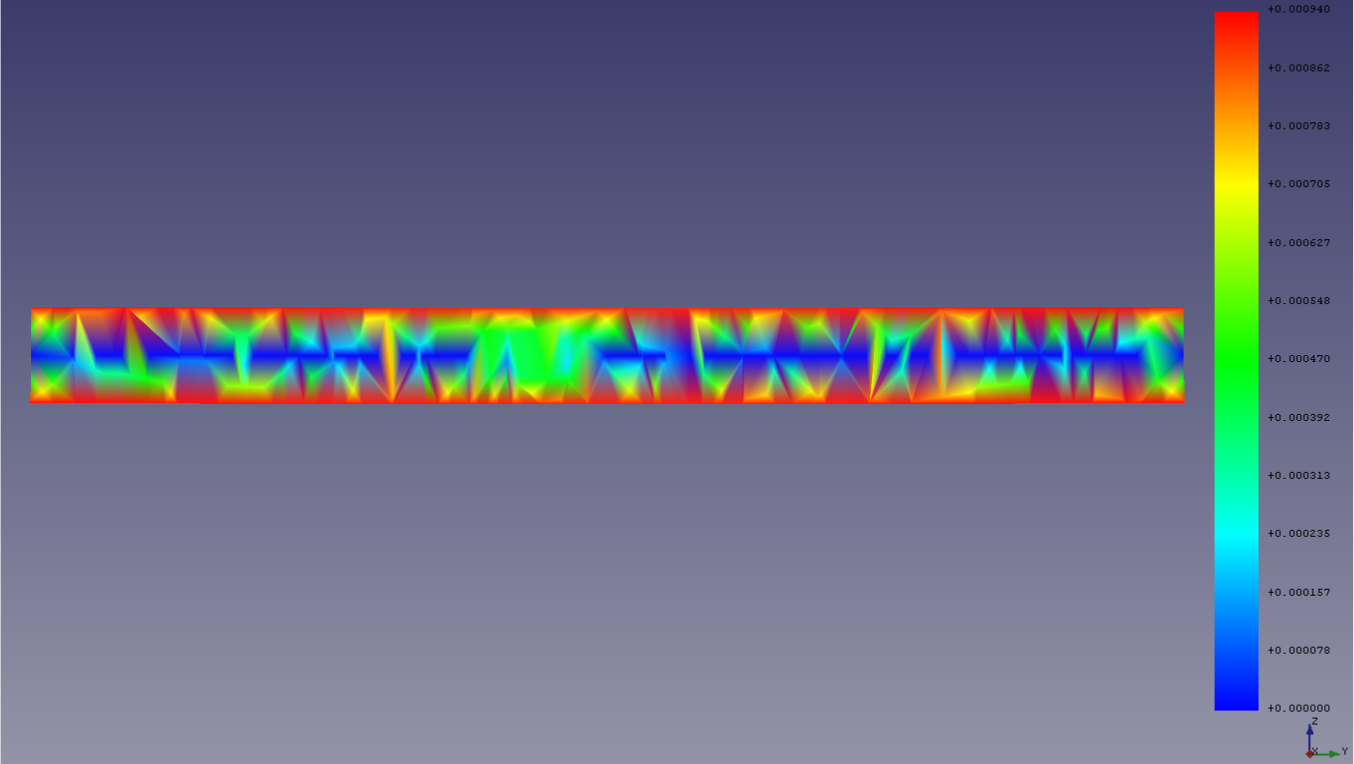
\includegraphics[width=\textwidth]{figures/resultados/strain_vector_magnitude_20.pdf}
    \caption{Distribución de la norma de la deformación $(\norm{\vec{\varepsilon}_{e_1}})$ en el plano de corte $\Pi$. Rango de la escala: $[0.000, \ 9.40] \times 10^{-3}$. Tamaño máximo de un elemento de malla: $2.0 \ \milli\meter$.}
    \label{fig:strain_vector_magnitude_20}
\end{figure}

Tal como sugiere \cite{manualPractica1} en la realización de la práctica, solamente se tendrá en cuenta la componente $\varepsilon_{11}$ para el cálculo de la deformación nominal. De igual forma que con la tensión, se promedian los valores de la cara superior e inferior para minimizar el error. Se tiene que $\varepsilon_\text{superior} = 8.51 \times 10^{-4}$ y $\varepsilon_\text{inferior} = -8.51 \times 10^{-4}$, por lo tanto,
\[
    \varepsilon_{g,\text{numérica}} = 
    \frac{\abs{\varepsilon_\text{superior}} + \abs{\varepsilon_\text{inferior}}}{2} = 
    \frac{8.51 \times 10^{-4} + 8.51 \times 10^{-4}}{2} = 
    8.51 \times 10^{-4}
\]

El error relativo entre deformación analítica y numérica se obtiene con la expresión análoga de \eqref{eq:error_relativo_tension}, sustituyendo tensiones por deformaciones,
\[
    \text{error}[\%] = 
    100 \ 
    \frac{
    \abs{\abs{\varepsilon_{g,\text{analítica}}} - \abs{\varepsilon_{g,\text{numérica}}}}}{\abs{\varepsilon_{g,\text{analítica}}}} = 
    100 \ \abs{\frac{8.3491 \times 10^{-4} - 8.51 \times 10^{-4}}{8.3491 \times 10^{-4}}} = 
    1.927 \%
\]
que es menor que $5 \%$, por lo que se toma como aceptable.


\subsection{Desplazamiento en \texorpdfstring{$z$}{z} en el punto de aplicación de la carga}

El desplazamiento en $Z$ en el punto de aplicación de la carga se obtiene analíticamente mediante
\begin{equation} \label{eq:desplazamiento_total_z}
    f = \frac{1}{3} \frac{P L_\text{total}^3}{E I}
\end{equation}
donde $L_\text{total} = L_g + 50 \ \milli\meter$ es la longitud total de la pieza e $I$ es el segundo momento de área de la sección transversal, dado por
\begin{equation} \label{eq:inercia}
    I = \frac{1}{12} b t^3
\end{equation}
Sustituyendo en \eqref{eq:inercia} con los datos de geometría de la Tabla \ref{tab:datos}, se tiene
\[
    I = 
    \frac{1}{12} \ 42 \ \milli\meter \cdot (3.5 \ \milli\meter)^3 = 
    150.0625 \ {\milli\meter}^4
\]
y el desplazamiento analítico,
\[
    f_\text{analítico} = 
    \frac{1}{3} 
    \frac{26 \ \newton \cdot (190 \ \milli\meter + 50 \ \milli\meter)^3}{69 \times 10^{3} \ \mega\pascal \cdot 150.0625 \ {\milli\meter}^4} = 
    11.571 \ \milli\meter
\]

En la Figura \ref{fig:displacement_vector_z_20_3d} se representa el desplazamiento en $z$ a lo largo de la probeta. Como resulta intuitivo, el mayor desplazamiento se produce en el extremo libre, mientras que cerca del empotramiento, a causa de la condición de contorno, el desplazamiento es nulo.
\begin{figure}[H]
    \centering
    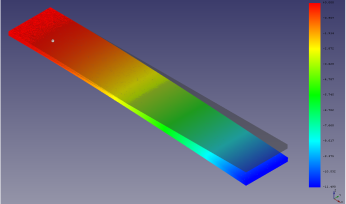
\includegraphics[width=\textwidth]{figures/resultados/displacement_vector_z_20_3d.pdf}
    \caption{Distribución de los desplazamientos en $z$. $\text{Warp Factor} = 1$. Rango de la escala: $[-11.490, \ 0.000] \ \milli\meter$. Tamaño máximo de un elemento de malla: $2.0 \ \milli\meter$.}
    \label{fig:displacement_vector_z_20_3d}
\end{figure}

En el extremo libre se tiene un desplazamiento numérico de
\[
    f_\text{numérico} = 11.490 \ \milli\meter
\]
por lo tanto el error relativo es
\[
    \text{error}[\%] = 
    100 \ \frac{\abs{ \abs{f_\text{analítico}} - \abs{f_\text{numérico}}} }{\abs{f_\text{analítico}}} = 0.691 \%
\]
Dado que es menor al $1\%$, la solución numérica y analítica están muy cerca.


\subsection{Carga máxima aplicable y coeficiente de seguridad} \label{sec:carga_maxima_aplicable_y_coeficiente_de_seguridad}

Supóngase que el límite elástico del material es $\sigma_e = 176 \ \mega\pascal$ y que se desea trabajar con un coeficiente de seguridad de $2$, a saber,
\begin{equation} \label{eq:coeficiente_seguridad}
    \text{Coeficiente de seguridad} = 
    \frac{\sigma_e}{\sigma_\text{máx}} = 2
\end{equation}
Para hallar la carga máxima aplicable $P_\text{máx}$, se opera con las Expresiones \eqref{eq:tension_analitica_galga} y \eqref{eq:coeficiente_seguridad} para obtener:
\begin{equation} \label{eq:carga_maxima}
    P_\text{máx} = \frac{1}{12} \frac{b t^2}{L_g} \sigma_e
\end{equation}
Como sugiere la Ecuación \eqref{eq:carga_maxima}, resulta intuitivo que a mayor ancho o grosor de probeta, mayor sea la carga máxima aplicable, pues más difícil será provocar la flexión. En cambio, a mayor longitud de probeta, menor es la carga máxima, dada la mayor facilidad para deformarla. Sustituyendo en \eqref{eq:carga_maxima} por los valores conocidos se tiene
\[
    P_\text{máx} = 
    \frac{1}{12} \frac{42 \ \milli\meter \cdot (3.5 \ \milli\meter)^2}{190 \ \milli\meter} \ 176 \ \mega\pascal = 
    39.72 \ \newton
\]

Una vez obtenida la carga máxima aplicable, se desea calcular con qué coeficiente de seguridad real está operando la pieza en la galga y en toda la pieza. Como tensiones ``reales'' se toman las obtenidas numéricamente. Recuérdese que en la galga $\sigma_{g,\text{numérica}} = 58.743 \ \mega\pascal$, de modo que el coeficiente de seguridad es
\[
    \text{Coeficiente de seguridad}_\text{galga} = 
    \frac{\sigma_e}{\sigma_{g,\text{numérica}}} = 
    \frac{176 \ \mega\pascal}{58.743 \ \mega\pascal} = 
    2.996
\]
que es mayor a $2$, por lo que se encuentra en la región aceptable. A fin de obtener la tensión máxima en toda la pieza, se calcula la componente $x$ del vector tensión, tal como se muestra en la Figura \ref{fig:stress_vector_x_all}.
\begin{figure}[H]
    \centering
    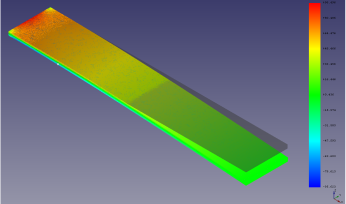
\includegraphics[width=\textwidth]{figures/resultados/stress_vector_x_all.pdf}
    \caption{Distribución de la componente $x$ del vector tensión en toda la probeta. Rango de la escala: $[-95.623, \ 96.496] \ \mega\pascal$. Tamaño máximo de un elemento de malla: $2.0 \ \milli\meter$.}
    \label{fig:stress_vector_x_all}
\end{figure}

\noindent
Se obtienen una tensión mínima de $\sigma_{\text{inferior}} = -95.623 \ \mega\pascal$, que se da en la cara inferior, y una tensión máxima de $\sigma_{\text{superior}} = 96.496 \ \mega\pascal$, que se da en la cara superior. Para obtener la tensión máxima en toda la pieza se promedian los valores anteriores:
\[
    \sigma_{\text{pieza,máxima}} = 
    \frac{\abs{\sigma_\text{inferior}} + 
    \abs{\sigma_\text{superior}}}{2} = 
    \frac{95.623 \ \mega\pascal + 96.496 \ \mega\pascal}{2} = 96.060 \ \mega\pascal
\]
De esta forma, el coeficiente de seguridad con el que opera la pieza es
\[
    \text{Coeficiente de seguridad}_\text{pieza} = 
    \frac{\sigma_e}{\sigma_{\text{pieza,máxima}}} = 
    \frac{176 \ \mega\pascal}{96.060 \ \mega\pascal} = 
    1.832
\]
que está muy por debajo de 2, por lo que es inadmisible. Para conseguir un coeficiente de seguridad mayor a $2$ es necesario reducir la carga $P$ en el extremo o bien modificar las dimensiones de la probeta.


\subsection{Estudio de la malla}

En todo problema resuelto de manera numérica es necesario estudiar cómo afectan los parámetros del método a la solución. En algunas situaciones este estudio es sencillo y directo. Por ejemplo, es evidente que al resolver un sistema de ecuaciones diferenciales $\dot{x}(t) = f(t,x(t))$, $x(t_0) = x_0$ con un método de Runge--Kutta de orden 5, los errores local y global serán mucho menores que al resolverlo con el método de Euler de orden 1, aunque ambos utilicen el mismo paso de tiempo $h$. En otros situaciones, por el contrario, esta relación no es tan directa o clara. Por ejemplo, si se resuelve la ecuación del calor en un dominio $\Omega \subset \real^3$ complicado, una malla no estructurada puede ser más adecuada que una estructurada. 

En el caso de estudio, el parámetro que puede modificarse y por lo tanto afectar a la solución es el tamaño máximo de un elemento de la malla. A continuación se lleva a cabo cómo afecta a los errores relativos y a los tiempos de resolución usando tamaños máximos de elementos de malla de $1.8 \ \milli\meter$ y $2.2 \ \milli\meter$.

\subsubsection{Efecto en los errores relativos}

En las siguientes figuras se muestran por pares las variables de estudio para los tamaños máximos de elementos de malla considerados. El procedimiento seguido para obtenerlos es el mismo que el seguido en las secciones anteriores, es decir, se corta la pieza deformada con el plano $\Pi \colon x = 50 \ \milli\meter$, y en la sección resultante se representan la tensión normal $\sigma_{11}$ y la deformación normal $\varepsilon_{11}$. Más precisamente:
\begin{itemize}
    \item En las Figuras \ref{fig:stress_vector_x_18} y \ref{fig:stress_vector_x_22} se representan las distribuciones de tensión normal en el plano de corte $\Pi$, para tamaños máximos de $1.8 \ \milli\meter$ y $2.2 \ \milli\meter$, respectivamente.
    \item En las Figuras \ref{fig:strain_vector_x_18} y \ref{fig:strain_vector_x_22} se representan las distribuciones de deformación normal en el plano de corte $\Pi$, para tamaños máximos de $1.8 \ \milli\meter$ y $2.2 \ \milli\meter$, respectivamente.
    \item En las Figuras \ref{fig:displacement_vector_z_18_3d} y \ref{fig:displacement_vector_z_22_3d} se representan las distribuciones de desplazamiento en $z$ en toda la pieza, para tamaños máximos de $1.8 \ \milli\meter$ y $2.2 \ \milli\meter$, respectivamente.
\end{itemize}

\begin{figure}[H]
    \centering
    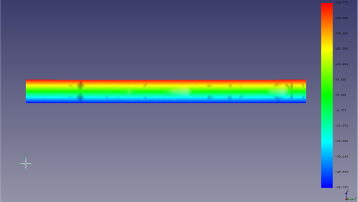
\includegraphics[width=\textwidth]{figures/resultados/stress_vector_x_18.pdf}
    \caption{Distribución de tensión normal $xx$ $(\sigma_{11})$ en el plano de corte $\Pi$. Rango de la escala: $[-58.747, \ 58.779] \ \mega\pascal$. Tamaño máximo de un elemento de malla: $1.8 \ \milli\meter$.}
    \label{fig:stress_vector_x_18}
\end{figure}

\begin{figure}[H]
    \centering
    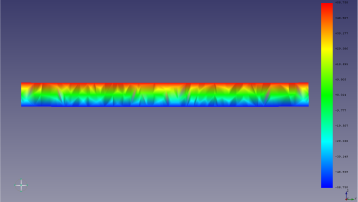
\includegraphics[width=\textwidth]{figures/resultados/stress_vector_x_22.pdf}
    \caption{Distribución de tensión normal $xx$ $(\sigma_{11})$ en el plano de corte $\Pi$. Rango de la escala: $[-58.730, \ 58.758] \ \mega\pascal$. Tamaño máximo de un elemento de malla: $2.2 \ \milli\meter$.}
    \label{fig:stress_vector_x_22}
\end{figure}

\begin{figure}[H]
    \centering
    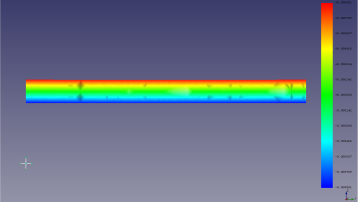
\includegraphics[width=\textwidth]{figures/resultados/strain_vector_x_18.pdf}
    \caption{Distribución de la deformación normal $xx$ $(\varepsilon_{11})$ en el plano de corte $\Pi$. Rango de la escala: $[-8.51, \ 8.51] \times 10^{-3}$. Tamaño máximo de un elemento de malla: $1.8 \ \milli\meter$.}
    \label{fig:strain_vector_x_18}
\end{figure}

\begin{figure}[H]
    \centering
    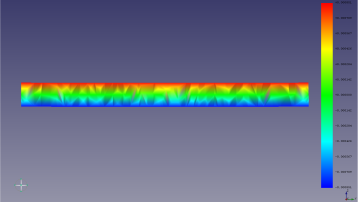
\includegraphics[width=\textwidth]{figures/resultados/strain_vector_x_22.pdf}
    \caption{Distribución de la deformación normal $xx$ $(\varepsilon_{11})$ en el plano de corte $\Pi$. Rango de la escala: $[-8.51, \ 8.51] \times 10^{-3}$. Tamaño máximo de un elemento de malla: $2.2 \ \milli\meter$.}
    \label{fig:strain_vector_x_22}
\end{figure}

\begin{figure}[H]
    \centering
    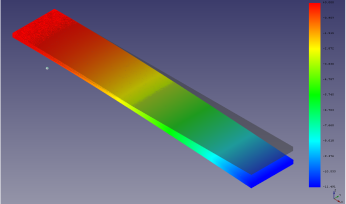
\includegraphics[width=\textwidth]{figures/resultados/displacement_vector_z_18_3d.pdf}
    \caption{Distribución de los desplazamientos en $z$. $\text{Warp Factor} = 1$. Rango de la escala: $[-11.491, \ 0.000] \ \milli\meter$. Tamaño máximo de un elemento de malla: $1.8 \ \milli\meter$.}
    \label{fig:displacement_vector_z_18_3d}
\end{figure}

\begin{figure}[H]
    \centering
    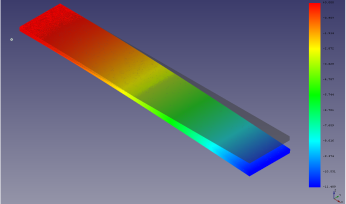
\includegraphics[width=\textwidth]{figures/resultados/displacement_vector_z_22_3d.pdf}
    \caption{Distribución de los desplazamientos en $z$. $\text{Warp Factor} = 1$. Rango de la escala: $[-11.489, \ 0.000] \ \milli\meter$. Tamaño máximo de un elemento de malla: $2.2 \ \milli\meter$.}
    \label{fig:displacement_vector_z_22_3d}
\end{figure}

Las distribuciones en todos los casos son similares. La única diferencia notable al cambiar el tamaño de máximo de elemento de malla es la ``suavidad'' en la transición de color. Las tensiones, deformaciones y desplazamientos, juntamente con los errores relativos para los tres tamaños de malla estudiados, se recogen en la Tabla \ref{tab:estudio_malla_error_relativo}.

\begin{table}[H]
    \centering
    \begin{tabular}{lccc}
        \toprule[0.50mm]
        \textbf{Variable} 
        & \textbf{Malla $\mathbf{1.8 \ mm}$} 
        & \textbf{Malla $\mathbf{2.0 \ mm}$} 
        & \textbf{Malla $\mathbf{2.2 \ mm}$} \\
        \midrule[0.25mm]
        Tensión superior $[\mega\pascal]$ & 
        \phantom{+}$58.779$ & 
        \phantom{+}$58.760$ & 
        \phantom{+}$58.758$ \\
        Tensión inferior \phantom{r}$[\mega\pascal]$ & 
        $-58.747$ & 
        $-58.726$ & 
        $-58.730$ \\
        Tensión \phantom{superior }$[\mega\pascal]$ & 
        \phantom{+}$58.763$ & 
        \phantom{+}$58.743$ & 
        \phantom{+}$58.744$ \\
        Err. rel. tensión & 
        \phantom{+}$2.003 \%$ & 
        \phantom{+}$1.968 \%$ & 
        \phantom{+}$1.970 \%$ \\
        \midrule[0.25mm]
        Deformación superior & 
        \phantom{+}$8.51 \times 10^{-4}$ & \phantom{+}$8.51 \times 10^{-4}$ & \phantom{+}$8.51 \times 10^{-4}$ \\
        Deformación inferior & 
        $-8.51 \times 10^{-4}$ & $-8.51 \times 10^{-4}$ & $-8.51 \times 10^{-4}$ \\
        Deformación & 
        \phantom{+}$8.51 \times 10^{-4}$ & \phantom{+}$8.51 \times 10^{-4}$ & \phantom{+}$8.51 \times 10^{-4}$ \\
        Err. rel. deformación & 
        $1.927 \%$ & $1.927 \%$ & $1.927 \%$ \\
        \midrule[0.25mm]
        Desplazamiento en $z$ $[\milli\meter]$ & 
        $11.491$ & $11.490$ & $11.489$ \\
        Err. rel. desplazamiento en $z$  & 
        $0.691 \%$ & $0.700 \%$ & $0.709 \%$ \\
        \bottomrule[0.50mm]
    \end{tabular}
    \caption{Variables de estudio y errores relativos para cada tamaño máximo de malla considerado.}
    \label{tab:estudio_malla_error_relativo}
\end{table}

\noindent
En lo que a tensiones se refiere, estas difieren ligeramente según el tamaño máximo de malla, siendo la máxima diferencia de errores relativos de $0.035 \%$. De manera intuitiva, una malla más fina debería dar errores relativos menores, es decir, la solución numérica debería estar más cerca a la solución analítica. No obstante, recuérdese que en la solución analítica es necesario hacer suposiciones y aproximaciones, por lo que esta última no es la solución real. En consecuencia, no es de extrañar que la solución con tamaño máximo de $1.8 \ \milli\meter$ esté más alejada de la analítica que la solución con tamaño máximo de $2.0 \ \milli\meter$. 

En cuanto a deformaciones, los errores relativos son iguales en todos los casos. Con toda seguridad las deformaciones difieren en algún punto a partir del sexto decimal. Sin embargo, esto no puede comprobarse, pues FreeCAD muestra como mucho seis decimales.

Finalmente, en cuanto a desplazamientos, los errores relativos son similares, aunque crecen ligeramente a medida que aumenta el tamaño máximo de malla. 

\subsubsection{Efecto en los tiempos de mallado y cálculo}

La discretización del dominio de estudio y cuán fina es afecta, por lo general, al tiempo de resolución. A fin de estudiar el efecto del tamaño máximo del elemento de malla en el tiempo de mallado y en el tiempo de cálculo, para cada tamaño se ha mallado y resuelto el problema diez veces. Posteriormente se ha calculado el promedio de tiempos. En las Tablas \ref{tab:tiempo_mallado} y \ref{tab:tiempo_calculo} se recogen los tiempos de mallado y de cálculo, respectivamente.

El tiempo de mallado crece rápidamente a medida que se reduce el tamaño máximo del elemento de malla. Es intuitivo que, a cuando crece el tamaño máximo del elemento de malla, el tiempo de mallado disminuye. Por consiguiente, si $\Delta x$ denota el tamaño máximo, el tiempo de mallado podría seguir una ley $t \propto 1 / {(\Delta x)}^\alpha$ para algún $\alpha > 0$. Para contrastar esto, no obstante, son necesarios más datos.

El comportamiento del tiempo de cálculo es similar al del tiempo de mallado, aunque en este caso el crecimiento al reducir el tamaño de malla es más acusado. 

\begin{table}[t]
    \centering
    \begin{tabular}{cccccccccccccc}
        \toprule[0.50mm]
        \textbf{Malla} & 
        \multicolumn{10}{c}{\textbf{Tiempo de mallado [s]}} & 
        \textbf{Promedio [s]} \\
        \midrule[0.25mm]
        $1.8 \ \milli\meter$ &
        $9.0$ & $9.0$ & $9.1$ & $9.0$ & $9.1$ & $9.0$ & $9.1$ & $9.0$ & 
        $9.0$ & $9.1$ & $9.0$ \\
        $2.0 \ \milli\meter$ & 
        $7.1$ & $7.1$ & $7.1$ & $7.1$ & $7.1$ & $7.0$ & $7.1$ & $7.0$ & 
        $7.0$ & $7.0$ & $7.1$ \\
        $2.2 \ \milli\meter$ & 
        $6.3$ & $6.2$ & $6.3$ & $6.4$ & $6.3$ & $6.2$ & $6.4$ & $6.4$ & 
        $6.4$ & $6.4$ & $6.3$ \\
        \bottomrule[0.50mm]
    \end{tabular}
    \caption{Tiempos de mallado y promedio de tiempos según el tamaño máximo de elemento de malla.}
    \label{tab:tiempo_mallado}
\end{table}

\begin{table}[t]
    \centering
    \begin{tabular}{cccccccccccccc}
        \toprule[0.50mm]
        \textbf{Malla} & 
        \multicolumn{10}{c}{\textbf{Tiempo de cálculo [s]}} & 
        \textbf{Promedio [s]} \\
        \midrule[0.25mm]
        $1.8 \ \milli\meter$ &
        $26.0$ & $25.9$ & $26.0$ & $26.0$ & $26.2$ & $26.1$ & $26.2$ & $26.0$ & 
        $26.1$ & $26.1$ & $26.1$ \\
        $2.0 \ \milli\meter$ & 
        $13.9$ & $14.0$ & $14.0$ & $14.1$ & $14.3$ & $14.2$ & $14.3$ & $14.3$ & 
        $14.4$ & $14.4$ & $14.2$ \\
        $2.2 \ \milli\meter$ & 
        $10.6$ & $10.6$ & $10.7$ & $10.7$ & $10.8$ & $10.9$ & $10.9$ & $11.0$ & 
        $11.1$ & $11.1$ & $10.8$ \\
        \bottomrule[0.50mm]
    \end{tabular}
    \caption{Tiempos de cálculo y promedio de tiempos según el tamaño máximo de elemento de malla.}
    \label{tab:tiempo_calculo}
\end{table}

El motivo por el que los tiempos crecen cuando $\Delta x$ disminuye es sencillo. Sea $V$ el volumen del dominio a mallar. Se puede asumir que el volumen del elemento de malla $V_e$ es proporcional al cubo del tamaño máximo, es decir, $V_e = k (\Delta x)^3$, para algún $k \in \real_{> 0}$. El número total de elementos en los que se discretiza el dominio es $N = V / (k (\Delta x)^3)$. Sea $c$ el número de variables asociadas a cada elemento de malla, de manera que en total se tienen $n = c V / (k (\Delta x)^3)$ variables. Supóngase que se quiere afinar la malla tomando $\Delta x' = \lambda \Delta x$ para $\lambda \in (0, 1)$. El número de variables para el problema con malla más fina es
\[
    n' = \frac{c V}{k (\Delta x')^3} = 
    \frac{1}{\lambda^3} \frac{c V}{k (\Delta x)^3} = 
    \frac{n}{\lambda^3}
\]
de donde se deduce que el número de variables total aumenta con el cubo de $\lambda^{-1}$. Si debe resolverse un sistema lineal, puede usarse, por ejemplo, la factorización LU. El número de operaciones que lleva a cabo este algoritmo es $\mathcal{O}(m^3)$, donde $m$ es la dimensión del sistema lineal a resolver. Para la malla de tamaño $\Delta x$ el número de operaciones es $\mathcal{O}(n^3)$, mientras que para la malla más fina de tamaño $\Delta x'$ este número crece a $\mathcal{O}(\lambda^{-9} n^3)$. En consecuencia, reducir a la mitad el tamaño de malla es prohibitivo en algunos casos. Todo y con esto, algunas propiedades de la matriz del sistema pueden aprovecharse para aplicar algoritmos más eficientes en número de operaciones, \eg si la matriz es simétrica.
